\documentclass[a4paper,norsk]{article}
\usepackage[latin1]{inputenc}
\usepackage[T1]{fontenc}
\usepackage{babel,textcomp,listings, subfigure,graphicx}
\usepackage{amsmath}
                                    
\title{Mandatory assignment 2, MEK4300}
\author{Sebastian Gjertsen}
\begin{document}
\maketitle
\section*{i}
\subsection*{a)}
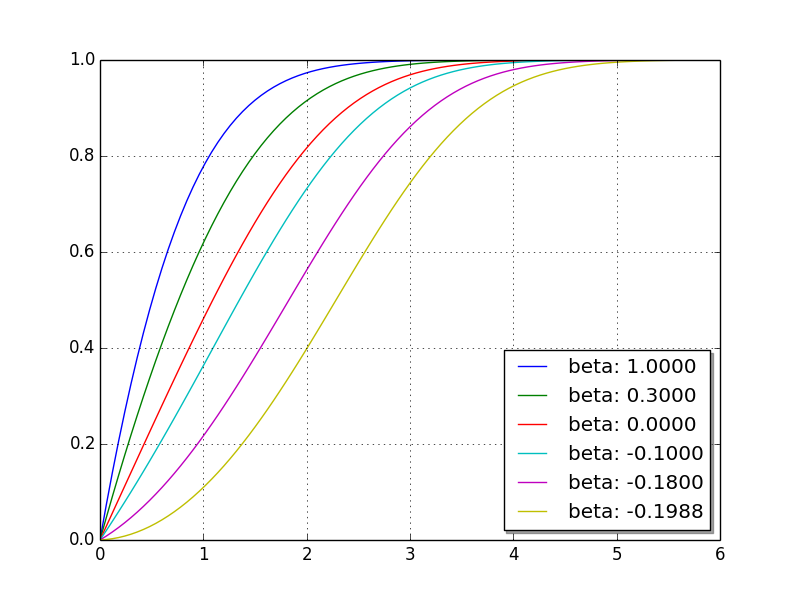
\includegraphics[trim = 0mm 0mm 0mm 0mm, clip, scale=0.3]{f_derivative.png} 
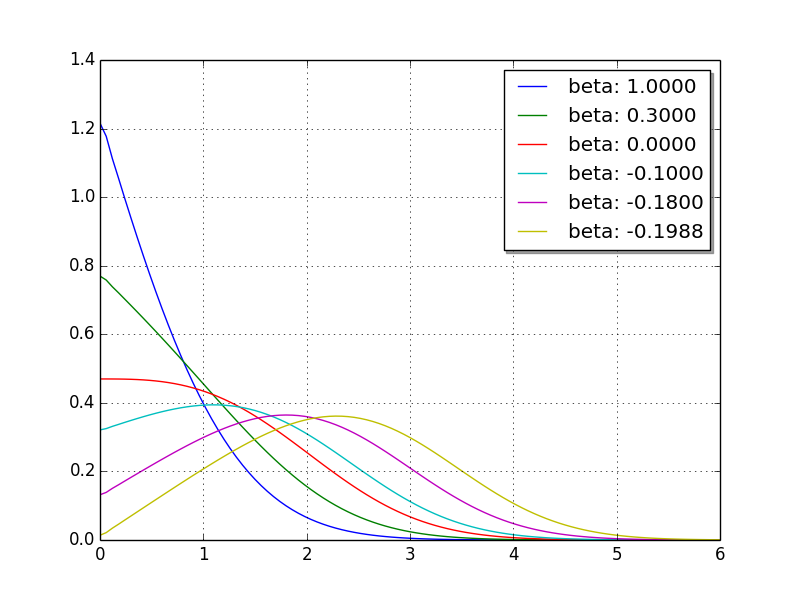
\includegraphics[trim = 0mm 0mm 0mm 0mm, clip, scale=0.3]{f_double_derivative.png} 
In the first section I have reproduced figure 4-11 in White, with different $beta$ values


\subsection*{b)}
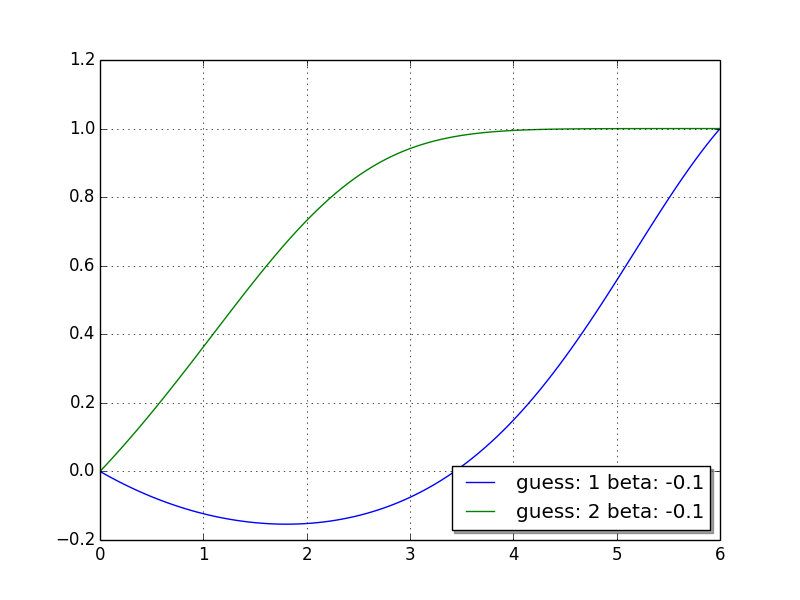
\includegraphics[trim = 0mm 0mm 0mm 0mm, clip, scale=0.3]{guess.png} 
The two guesses in the plots are with (0,0) and (1,1)

\section*{ii}
\subsection*{a)}
In the first test with steady solver and Re = 20
$$C_D= 5.79392133271, C_L = 0.00871442276844, \Delta P = 0.11435196$$
which is pretty close compare to the benchmark :$$C_D =  5.5567 , C_L = 0.0106 , \Delta P =  0.1172 $$
\subsection*{b)}
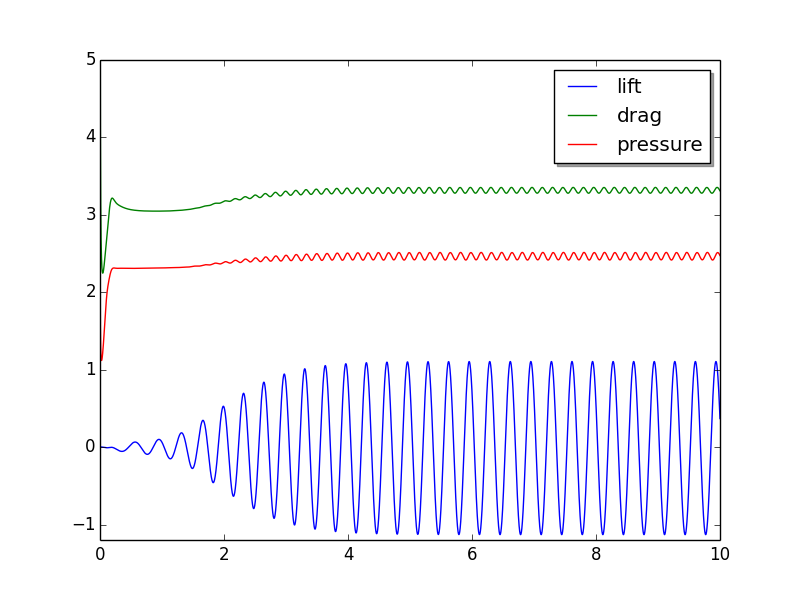
\includegraphics[trim = 0mm 0mm 0mm 0mm, clip, scale=0.4]{lift_drag_pressure_plot.png} 
\newline
To compute the flow past the cylinder I used Chorins method to discretize the Navier-Stokes Equations. This method solves NS in the 3 steps
Using $dt = 0.0005 $ and a mesh with:  117531 degrees of freedom
We can see from the plot that the lift, pressure and drag oscillates as the fluid moves past the cylinder. This is because the cylinder is uncentered making the fluid move faster on one side. And with a high enough Reynolds number the system tries to equalize and then these oscillations begin.

\begin{tabular}{l*{6}{c}r}
 &$CL_max$  & $Cd_max   $ & $ \Delta p $   \\
\hline
Me & 1.1055 & 3.3542 & 2.5144 \\
Turek et al & 0.9672 & 3.2224 & 2.4814 \\
\end{tabular}

\section*{iii}
\subsection*{a)}
The first thing we do is to assume that the pressure gradient in the x direction is constant and see what we can do:
$$ \frac{1}{\rho} \frac{\partial \bar{p}}{\partial x} = \nu \frac{\partial^2 \bar{u}}{\partial y^2} - \frac{\partial \overline{u'v'}}{\partial y}    $$
If we then integrate this rhs hans side with respect to y from 0 to 1, the last term vanishes since both functions are zero on each wall.
The other term can we see is the same as $(v^*)^2 = 0.025$. We then have a value for $$ \frac{1}{\rho} \frac{\partial \bar{p}}{\partial x} $$
Since the problem in constant in the x direction we can solve it in 1D. And since it is symmetric from the midpoint out. We need only solve half of the domain. Putting Dirichlet equal to zero on the wall and Neumann on the other end.

To make sure that we have enough nodes towards the wall $y^+ < 1$, this means that on a unit interval mesh we will need 1001 points since $ y^+ = y*1000$ 

\subsection*{b)}
We see from the first plot that our solution matches very well for $y^+<5$ and is pretty good for $y^+>30$. After some trial and error i got that $B = 5.16$ gives the best approximation with the computational results. \newline
The last plot is of $\nu_t$ over our domain which at the end of the plot is which is in the middle of the channel. This signifies that there is no turbulence in the middle of the channel which does not seem reasonable. Since we would expect there to be a rlot of turbulence in the middle of a turbulent channel. This signifies the shortcomings of the model. \newline
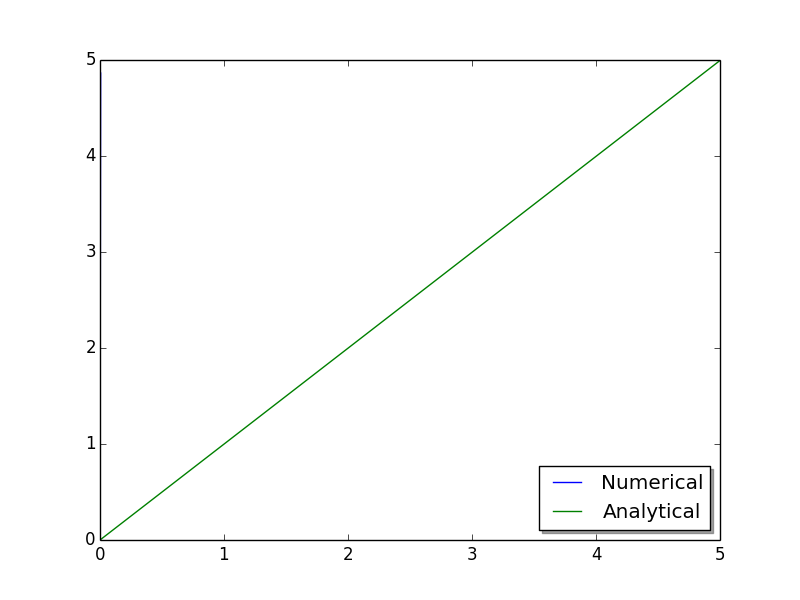
\includegraphics[trim = 0mm 0mm 0mm 0mm, clip, scale=0.3]{error_5.png} 
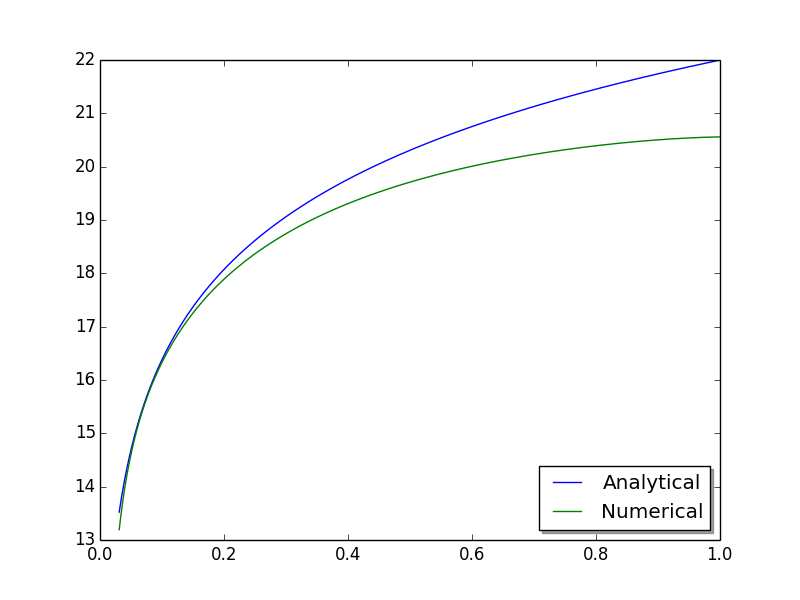
\includegraphics[trim = 0mm 0mm 0mm 0mm, clip, scale=0.3]{error_30.png} 
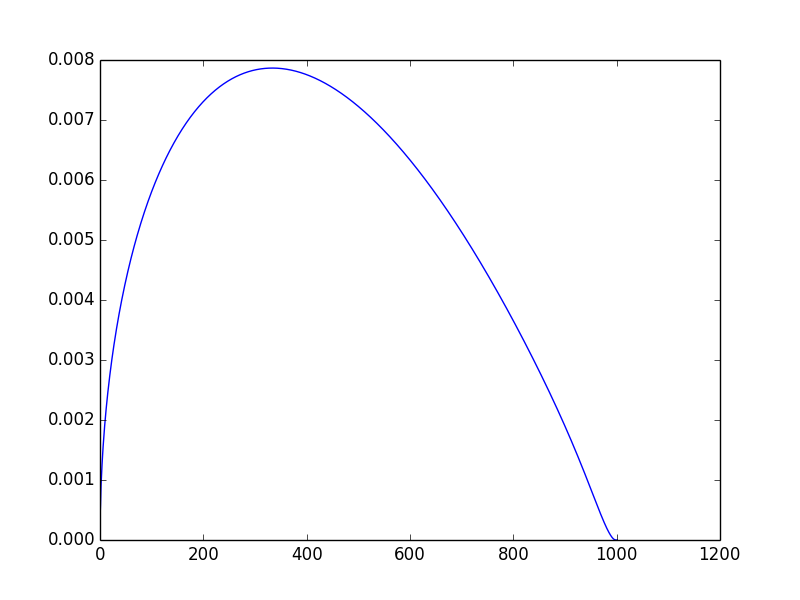
\includegraphics[trim = 0mm 0mm 0mm 0mm, clip, scale=0.3]{nu_t.png} 



\section*{iv}
\subsection*{RANS}
To get the RANS equations we start with the Navier-Stokes equations and split up the velocity into a mean and fluctuating part $ u = \bar{u} + u^{'} $
N-S:
\begin{equation}
 \frac{\partial u_i}{\partial t} + u_j \frac{\partial u_i}{\partial x_j} = - \frac{1}{\rho} \frac{\partial p}{\partial x_i} + \nu \frac{\partial^2 u_i}{\partial x_j^2}    
\end{equation}
If we then take the mean of every term we get:
\begin{align*}
\overline{\frac{\partial u_i}{\partial t}} &= \frac{\partial \overline{u_i}}{\partial t}\\
\overline{\frac{1}{\rho} \frac{\partial p}{\partial x_i}} &= \frac{1}{\rho} \frac{\partial \bar{p}}{\partial x_i} \\
\overline{\nu \frac{\partial^2 u_i}{\partial x_j^2}} &= \nu \frac{\partial^2 \bar{u_i}}{\partial x_j^2}  \\
u_j \frac{\partial u_i}{\partial x_j} &= \frac{\partial u_iu_j}{\partial x_j} - u_i \frac{\partial u_j}{\partial x_j}\\
& \text{where this last term is zero because of incompressibility}\\
\overline{u_i u_j} & = \overline{u_i u_j} + \overline {u_i^{'}u_j^{'}} \\
\text{since  } \bar{u} &= \overline{\bar{u}+u^{'}} = \bar{u}\\
\overline{u_j \frac{\partial u_i}{\partial x_j}} =& \frac{\partial (\overline{u_iu_j} + u_i^{'}u_j^{'})}{\partial x_j} = \bar{u_j} \frac{\partial \bar{u_i}}{\partial x_j} + \frac{\partial u_i^{'} u_j^{'}}{\partial x_j}
\end{align*}
Putting all this together we get:
\begin{equation}
\frac{\partial \overline{u_i}}{\partial t} +\bar{u_j} \frac{\partial \bar{u_i}}{\partial x_j}  =- \frac{1}{\rho} \frac{\partial \bar{p}}{\partial x_i}+  \nu \frac{\partial^2 \bar{u_i}}{\partial x_j^2} + \frac{\partial u_i^{'} u_j^{'}}{\partial x_j}
\end{equation}
$$ \frac{\partial \bar{u_i}}{\partial x_i} = 0 $$

\subsection*{Reynolds Stress Equation}
We start by taking NS minus RANS (1)-(2) giving, term by term:
\begin{align*}
\frac{\partial u_i}{\partial t} - \frac{\partial \bar{u_i}}{\partial t} &= \frac{\partial u^{'}_i}{\partial t}\\
u_j \frac{\partial u_i}{\partial x_j} &= \frac{\partial u_iu_j}{\partial x_j} \\
\bar{u_j} \frac{\partial \bar{u_i}}{\partial x_j} &= \frac{\partial \bar{u_i}\bar{u_j}}{\partial x_j} \\
\frac{\partial \bar{u_i}\bar{u_j}}{\partial x_j} - \frac{\partial \bar{u_i}\bar{u_j}}{\partial x_j} &= \frac{\partial }{\partial x_j} (\bar{u_i}\bar{u_j} + u^{'}_i\bar{u_j} + \bar{u_i}u^{'}_j + u^{'}_i u{'}_j -\bar{u_i}\bar{u_j} )\\
\nu \frac{\partial^2 u_i}{\partial x_j^2} - \nu \frac{\partial^2 \bar{u_i}} {\partial x_j^2} &= \nu \frac{\partial^2 u^{'}_i} {\partial x_j^2} \\
\frac{1}{\rho}\frac{\partial p} {\partial x_i} - \frac{1}{\rho}\frac{\partial \bar{p}} {\partial x_i} = \frac{1}{\rho}\frac{\partial p^{'}} {\partial x_i}
\end{align*}
If we put these together and use the product rule trick we used above we get:
\begin{align*}
\frac{\partial u^{'}_i}{\partial t} + \bar{u_j} \frac{\partial u^{'}_i}{\partial x_j} &= - \frac{1}{\rho}\frac{\partial p^{'}} {\partial x_i} + \nu \frac{\partial^2 u^{'}_i} {\partial x_j^2} - u^{'}_j \frac{\partial \bar{u}_i}{\partial x_j} - 
u^{'}_j \frac{\partial u^{'}_i}{\partial x_j}  + \overline{u^{'}_j \frac{\partial u^{'}_i}{\partial x_j}}   \\
\end{align*}
We time this equation with $u_k^{'}$
\begin{equation}
u_k^{'}\frac{\partial u^{'}_i}{\partial t} + u_k^{'}\bar{u_j} \frac{\partial u^{'}_i}{\partial x_j} = - u_k^{'}\frac{1}{\rho}\frac{\partial p^{'}} {\partial x_i} + u_k^{'}\nu \frac{\partial^2 u^{'}_i} {\partial x_j^2} - u_k^{'}u^{'}_j \frac{\partial \bar{u}_i}{\partial x_j} - u_k^{'}u^{'}_j \frac{\partial u^{'}_i}{\partial x_j}  + u_k^{'}\overline{u^{'}_j \frac{\partial u^{'}_i}{\partial x_j}}   \\
\end{equation}
We look at the inverted of this equation:
\begin{equation}
u_i^{'}\frac{\partial u^{'}_k}{\partial t} + u_i^{'}\bar{u_j} \frac{\partial u^{'}_k}{\partial x_j} = - u_i^{'}\frac{1}{\rho}\frac{\partial p^{'}} {\partial x_k} + u_i^{'}\nu \frac{\partial^2 u^{'}_k} {\partial x_j^2} - u_i^{'}u^{'}_j \frac{\partial \bar{u}_k}{\partial x_j} - u_i^{'}u^{'}_j \frac{\partial u^{'}_k}{\partial x_j}  + u_i^{'}\overline{u^{'}_j \frac{\partial u^{'}_k}{\partial x_j}}   \\
\end{equation}
We take (1) + (2) and look at each term:
The first thing we get when looking at the two left most terms, and apply the product rule, is: 
$$   u_k^{'}\frac{\partial u^{'}_i}{\partial t} +   u_i^{'}\frac{\partial u^{'}_k}{\partial t} = \frac{\partial \overline{u_i^{'}u_k^{'}}}{\partial t} $$
$$ u_k^{'}\bar{u_j} \frac{\partial u^{'}_i}{\partial x_j}  + u_i^{'}\bar{u_j} \frac{\partial u^{'}_k}{\partial x_j} = \bar{u_j}\frac{\partial \overline{u_i^{'}u_k^{'}}}{\partial t}  $$
And these two together can be written as:
$$ \frac{D \overline{u_i^{'}u_k^{'}}}{Dt} $$
which makes our left hand side.
We then look at the pressure terms:
we can write the pressure using product rule as:
$$ \frac{1}{\rho}\frac{\partial}{\partial x_i} (p^{'} u_k^{'}) = \frac{1}{\rho}u_k^{'} \frac{\partial p^{'} }{\partial x_i} - \frac{1}{\rho}p{'} \frac{\partial u_k^{'} }{\partial x_i}    $$
$$ \frac{1}{\rho}\frac{\partial}{\partial x_k} (p^{'} u_i^{'}) = \frac{1}{\rho}u_i^{'} \frac{\partial p^{'} }{\partial x_k} - \frac{1}{\rho}p{'} \frac{\partial u_i^{'} }{\partial x_k}    $$

\begin{align*}
- u_k^{'}\frac{1}{\rho}\frac{\partial p^{'}} {\partial x_i} - - u_i^{'}\frac{1}{\rho}\frac{\partial p^{'}} {\partial x_k} &=  -\frac{1}{\rho}\frac{\partial}{\partial x_k} (p^{'} u_i^{'}) +  \frac{1}{\rho}p{'} \frac{\partial u_i^{'} }{\partial x_k} - \frac{1}{\rho}\frac{\partial}{\partial x_i} (p^{'} u_k^{'}) + \frac{1}{\rho}p{'} \frac{\partial u_k^{'} }{\partial x_i} \\
 & =\frac{1}{\rho}\big( \frac{\partial u^{'}_i}{\partial x_k} + \frac{\partial u^{'}_k}{\partial x_i} \big) - \frac{1}{\rho}\frac{\partial}{\partial x_i} (p^{'} u_k^{'}) - \frac{1}{\rho}\frac{\partial}{\partial x_k} (p^{'} u_i^{'}) \\
 &=  \frac{1}{\rho}\big( \frac{\partial u^{'}_i}{\partial x_k} + \frac{\partial u^{'}_k}{\partial x_i} \big) -\frac{1}{\rho} \frac{\partial}{\partial x_j} ( p^{'}( \delta_{ij} u_k + \delta_{kj}u_i    )     )
\end{align*}
Next is the term with $\nu$, we again use the product rule:
\begin{equation*}
u_k^{'}\nu \frac{\partial^2 u^{'}_i} {\partial x_j^2} + u_i^{'}\nu \frac{\partial^2 u^{'}_k} {\partial x_j^2} = \nu \frac{\partial^2 u^{'}_i u^{'}_k}{\partial x_j^2} - 2\nu \frac{\partial u^{'}_i }{\partial x_j} \frac{\partial u^{'}_k }{\partial x_j}
\end{equation*}
Lastly:
\begin{equation*}
u_k^{'}u_j^{'}\frac{\partial u_i^{'}}{\partial x_j} + u_i^{'}u_j^{'}\frac{\partial u_k^{'}}{\partial x_j} = \frac{\partial u_i^{'} u_j^{'} u_k^{'}}{\partial x_j}
\end{equation*}
Putting all these together and taking the average of everything, we get what we wanted:

\begin{equation}
 \frac{D \overline{u_i^{'}u_k^{'}}}{Dt} = -\overline{ u_k^{'}u_j^{'}\frac{\partial u_i^{'}}{\partial x_j}} - \overline{u_i^{'}u_j^{'}\frac{\partial u_k^{'}}{\partial x_j}} -  \overline{2\nu \frac{\partial u^{'}_i }{\partial x_j} \frac{\partial u^{'}_k }{\partial x_j}}
 + \overline{\frac{1}{\rho}\big( \frac{\partial u^{'}_i}{\partial x_k} + \frac{\partial u^{'}_k}{\partial x_i} \big)} - \frac{\partial }{\partial x_k} \big[ \overline{u_i^{'} u_j^{'} u_k^{'}} -  \nu\overline{ \frac{\partial u^{'}_i u^{'}_k}{\partial x_j}} + 
     \overline{\frac{p^{'}}{\rho} ( \delta_{ij} u_k + \delta_{kj}u_i  )} \big]  
\end{equation}
\newline
\newline

\subsection{Kinetic-Energy Equation}
To get the Turbulence Kinetic-Energy equation. We start like before with NS - RANS, and times this equation with $u_i^{'}$.
We use the product rule like before and get term by term:
\begin{align*}
u_i^{'}\frac{\partial u_i^{'}}{\partial t} &= \frac{1}{2}\frac{\partial u_i^{'}u_i^{'}}{\partial t} \\
u_i^{'}u_j^{'} \frac{\partial u_i^{'}}{\partial x_j} &= \frac{1}{2}u_j^{'}\frac{\partial u_i^{'}u_i^{'}}{\partial x_j}
\end{align*}
We will call  $ K = \frac{1}{2}\overline{u_i^{'}u_i^{'}}$ 
These to together, and taking the mean, gives us the LHS:
$$ \frac{DK}{Dt}   $$
We already have the term:
$$  \overline{u_i^{'}u_j^{'}}\frac{\partial \bar{u_j}}{\partial x_j} $$ 
and 
$$ u_i^{'}\frac{\partial p^{'}}{\partial x_i} $$
To get the same as white we rewrite the second last term
$$\nu \frac{\partial }{\partial x_j} (u_i \frac{\partial u_i^{'}}{\partial x_j}) = \nu\frac{\partial u_i}{\partial x_j}\frac{\partial u_i}{\partial x_j} +\nu  u_i \frac{\partial^2 u_i}{\partial x_j^2}       $$
$$\nu \frac{\partial }{\partial x_j} (u_i \frac{\partial u_j^{'}}{\partial x_i}) =\nu \frac{\partial u_i}{\partial x_j}\frac{\partial u_j}{\partial x_i} + \nu u_i \frac{\partial u_j}{\partial x_i \partial x_j}       $$
we have from NS-RANS
$$\nu  u_i \frac{\partial^2 u_i}{\partial x_j^2}  $$
$$ \nu  u_i \frac{\partial^2 u_i}{\partial x_j^2} = \nu \frac{\partial u_i}{\partial x_j}\frac{\partial u_j}{\partial x_i} + \nu u_i \frac{\partial u_j}{\partial x_i \partial x_j}  +$$
$$  \nu\frac{\partial u_i}{\partial x_j}\frac{\partial u_i}{\partial x_j} - \nu \frac{\partial u_i}{\partial x_j}\frac{\partial u_j}{\partial x_i} - \nu u_i \frac{\partial u_j}{\partial x_i \partial x_j} $$















\end{document}
